\chapter{Decomposição em Valores Singulares}

A SVD é uma técnica fundamental em álgebra linear com aplicações em diversas áreas, como compressão de dados, processamento de imagens e solução de sistemas lineares. Este capítulo explora a utilização da SVD para fatoração e aproximação de matrizes grandes, com foco em imagens como caso prático.

\section{Fundamentos Matemáticos}

Seja \( A \) uma matriz de dimensões \( m \times n \). A SVD permite escrever \( A \) como o produto de três matrizes:
\begin{equation}
  A = U S V^\top,
\end{equation}
onde \( U \) é uma matriz ortogonal de dimensão \( m \times m \), cujas colunas são os vetores singulares à esquerda; \( S \) é uma matriz diagonal de dimensão \( m \times n \), contendo os valores singulares \( \sigma_1, \sigma_2, \dots, \sigma_r \) na diagonal, ordenados de forma decrescente (\( \sigma_1 \geq \sigma_2 \geq \dots \geq \sigma_r > 0 \)), sendo \( r \) o posto de \( A \); e \( V \) é uma matriz ortogonal de dimensão \( n \times n \), cujas colunas são os vetores singulares à direita.

A decomposição é possível para qualquer matriz \( A \), sem restrições de simetria ou de outros critérios. Isso distingue a SVD de outras técnicas de fatoração, como a diagonalização, que exige que a matriz seja quadrada e simétrica.

\subsection{Construção das Matrizes}

A matriz \( S \) contém os valores singulares de \( A \), que estão relacionados com as raízes quadradas dos autovalores das matrizes \( A^\top A \) e \( A A^\top \). Esses valores medem a importância das diferentes dimensões em \( A \) e desempenham papel central em aplicações de compressão e aproximação. As colunas de \( U \) e \( V \) são os vetores próprios de \( A A^\top \) e \( A^\top A \), respectivamente. Esses vetores definem bases ortonormais no domínio e na imagem da transformação linear associada a \( A \).

No processo de cálculo da SVD, primeiramente determina-se \( V \) multiplicando \( A \) por sua transposta \( A^\top \), resultando na matriz simétrica \( A^\top A \):
\begin{equation}
  A^\top A = V S^2 V^\top.
\end{equation}
Diagonalizando \( A^\top A \), os autovetores obtidos formam as colunas de \( V \), enquanto os autovalores são os quadrados dos valores singulares.

Em seguida, determina-se \( U \) de forma similar a matriz V. Neste caso, calcula-se \( A A^\top \), que também é simétrica:
\begin{equation}
  A A^\top = U S^2 U^\top.
\end{equation}
Os autovetores dessa matriz correspondem às colunas de \( U \).

Por fim, a matriz \( S \) é construída posicionando os valores singulares na diagonal principal, com as demais entradas iguais a zero.

\section{Aplicações em Processamento de Imagens}

A SVD é amplamente utilizada para compressão de imagens. Ao representar uma imagem como uma matriz de intensidades, os valores singulares maiores capturam a maior parte da informação visual. Assim, pode-se aproximar a matriz original com poucos valores singulares, reduzindo o espaço de armazenamento sem perda significativa de qualidade visual.

\subsection{Compressão de Imagens}

A compressão de imagens utilizando a SVD baseia-se na transformação de uma matriz \( A \), que representa a imagem, no formato \( A = U S V^\top \). O objetivo principal dessa transformação é reduzir o número de entradas necessárias para representar a matriz \( A \) sem comprometer significativamente a qualidade da informação.

Ao decompor \( A \) no produto \( U S V^\top \), é possível aproximar \( A \) utilizando uma versão de posto reduzido. Em termos práticos, essa redução remove informações redundantes, ou seja, aquelas que são linearmente dependentes. Assim, para um posto \( r \) menor que \( m \) ou \( n \) (as dimensões da matriz \( A \)), obtém-se uma matriz que captura a maior parte da essência estrutural de \( A \), minimizando a perda de informação relevante.

A matriz \( A \) pode ser reescrita como uma soma dos produtos externos escalados pelos valores singulares:
\[
  A = \sigma_1 u_1 v_1^\top + \sigma_2 u_2 v_2^\top + \cdots + \sigma_r u_r v_r^\top + \sum_{i=r+1}^p \sigma_i u_i v_i^\top,
\]
onde \( \sigma_i \) são os valores singulares ordenados em ordem decrescente (\( \sigma_1 \geq \sigma_2 \geq \cdots \geq \sigma_r > 0 \)) e \( u_i, v_i \) são os vetores singulares à esquerda e à direita, respectivamente.

Os valores singulares associados a índices maiores que o posto \( r \) são iguais a zero. Consequentemente, os termos correspondentes não contribuem para a matriz \( A \) e podem ser ignorados, resultando na seguinte aproximação:
\[
  A \approx \sum_{i=1}^r \sigma_i u_i v_i^\top.
\]

Além disso, mesmo os valores singulares menores (aqueles próximos a zero) podem ser desconsiderados para reduzir ainda mais o número de termos na soma. Como os valores singulares são dispostos em ordem decrescente, os termos associados a valores singulares menores têm impacto reduzido na estrutura geral de \( A \).

Ao descartar termos associados a valores singulares menores, a quantidade de dados necessária para representar a imagem é reduzida significativamente. Essa redução ocorre porque, em vez de armazenar todos os \( m \times n \) elementos de \( A \), armazenamos apenas os vetores singulares (\( u_i \) e \( v_i \)) e os valores singulares (\( \sigma_i \)) para \( i \leq k \), onde \( k \) é o número de termos retidos. Além disso, a precisão da aproximação pode ser ajustada variando \( k \). Retendo mais termos (\( k \) maior), preserva-se mais detalhes da imagem; ao reduzir \( k \), a compressão é maior, mas pode haver perda de qualidade.

\section{Exemplo Prático}


Para ilustrar o processo de compressão de imagens utilizando a SVD, considera-se uma imagem, apresentada na \autoref{fig:image},  representada por uma matriz \( A \). O objetivo é reduzir o posto da matriz \( A \) para obter versões aproximadas da imagem original, utilizando um número menor de valores singulares.

\begin{figure}
  \centering
  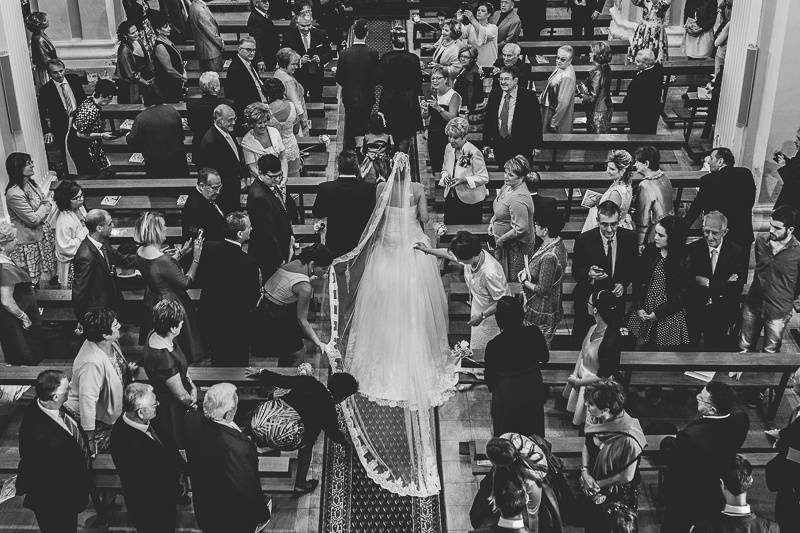
\includegraphics[width=.45\textwidth]{Figures/image.jpeg}
  \caption{Imagem original a ser compressada.}
  \label{fig:image}
\end{figure}

A matriz \( A \) foi fatorada no formato \( A = U S V^\top \). Em seguida, foram construídas aproximações de posto reduzido ao reter apenas os \( k \) maiores valores singulares e seus vetores singulares associados. Cada aproximação pode ser expressa como:
\begin{equation}
  A_k = \sum_{i=1}^k \sigma_i u_i v_i^\top,
\end{equation}
onde \( k \) é o posto escolhido.

As imagens apresentadas na \autoref{fig:result} ilustram os resultados da compressão para diferentes valores de posto \( k \), obtidas por meio do algoritmo implementado apresentado em \autoref{cod:a1}. Utilizando apenas os cinco maiores valores singulares (\( k = 5 \)), observa-se que a estrutura geral da imagem é visível, embora com perda significativa de detalhes. Quando o número de termos é aumentado para \( k = 20 \), os contornos e formas tornam-se mais definidos. Com \( k = 50 \), a imagem apresenta maior nitidez e detalhes perceptíveis, aproximando-se da qualidade do original. Finalmente, ao utilizar \( k = 100 \), a imagem se aproxima ainda mais da original, com uma perda mínima de qualidade. Esses resultados demonstram que os primeiros valores singulares capturam a maior parte das informações relevantes da imagem, permitindo que uma retenção reduzida de termos seja suficiente para reconstruir uma aproximação de boa qualidade, ao mesmo tempo em que reduz significativamente o espaço necessário para armazenamento.

\begin{figure}
  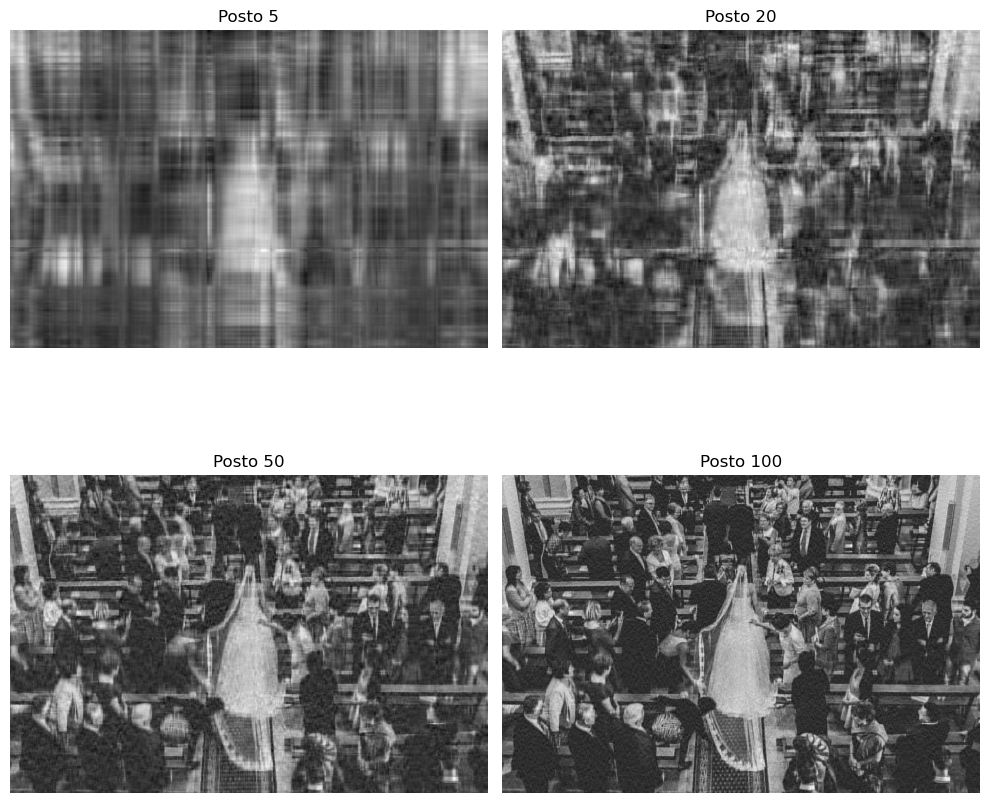
\includegraphics[width=1.\textwidth]{Figures/result.png}
  \caption{Resultados obtidos na compressão da imagem para postos iguais a 5, 20, 50 e 100.}
  \label{fig:result}
\end{figure}


Do ponto de vista da eficiência, a compressão oferece uma redução considerável na complexidade de armazenamento. Enquanto a imagem original, de posto completo, exige o armazenamento de \( m \times n \) entradas, uma aproximação de posto \( k \) requer apenas \( k (m + n + 1) \) entradas, devido ao armazenamento das colunas de \( U_k \), \( V_k^\top \) e dos valores \( \sigma_i \).